\documentclass[11pt,a4paper]{article}
\usepackage[T1]{fontenc}
\usepackage[utf8]{inputenc}
\usepackage[spanish]{babel}
\usepackage{lmodern}
\usepackage{geometry}
\usepackage{amsmath,amssymb}
\usepackage{booktabs}
\usepackage{longtable}
\usepackage{array}
\usepackage{tabularx}
\usepackage{graphicx}
\usepackage{float}
\usepackage{caption}
\usepackage{hyperref}
\usepackage{enumitem}
\geometry{margin=2.3cm}
\hypersetup{colorlinks=true,linkcolor=blue,urlcolor=blue,citecolor=blue}
\setlength{\parskip}{0.4em}
\setlength{\parindent}{0pt}

\title{Informe Integrado de Kernels, Bandwidths y Pruebas Estadisticas\\para \texttt{Kernel\_Tests}}
\author{Proyecto \texttt{Clustering\_Microbiota}}
\date{\today}

\begin{document}
\maketitle

\begin{abstract}
Este documento reemplaza el PDF previo \texttt{Analisis\_Correcciones\_MultiKernel.pdf} por una
version integrada y reproducible. El nuevo informe no solo corrige errores de la version anterior;
tambien resume el proceso real de los cuatro notebooks ejecutados, explicita que kernels se estan
usando en el flujo, propone valores comparables de bandwidth para los seis kernels disponibles y
agrega pruebas estadisticas complementarias sobre las distribuciones KDE. El foco del reporte es
operativo: dejar claro que configuraciones sirven como referencia tecnica, cuales quedan mejor
paradas para describir la distribucion de valores positivos y que limitaciones siguen abiertas.
\end{abstract}

\section{Alcance y archivos revisados}
Se revisaron y ejecutaron:
\begin{itemize}[leftmargin=1.5em]
\item \texttt{Kernel\_Tests/KDE\_Gridsize\_Sensitivity.ipynb}
\item \texttt{Kernel\_Tests/KDE\_Estadisticas.ipynb}
\item \texttt{Kernel\_Tests/KDE\_Estadisticas\_MultiKernel.ipynb}
\item \texttt{Kernel\_Tests/KDE\_Gridsize\_Sensitivity\_MultiKernel.ipynb}
\item \texttt{Kernel\_Tests/build\_kernel\_report\_assets.py}
\end{itemize}

El conjunto de datos \texttt{Datos/otu\_data\_converted.csv} contiene \(441\) muestras,
\(4738\) columnas numericas de OTUs y \(2{,}089{,}458\) entradas numericas. Tras aplanar la matriz
y descartar ceros, el flujo KDE trabaja con \(105{,}420\) valores positivos, con media
\(139.921\), mediana \(8\), desviacion estandar \(895.074\), minimo \(1\) y maximo \(60{,}711\).

\section{Unidad analizada y limitacion central}
Los notebooks no modelan una muestra biologica individual ni una abundancia por OTU aislada. El
objeto estadistico que realmente se esta analizando es la distribucion de todas las entradas
positivas de la matriz de conteos una vez aplanada. Esto tiene dos consecuencias importantes:
\begin{enumerate}[leftmargin=1.5em]
\item las conclusiones describen la distribucion condicional \(X \mid X > 0\), no la distribucion
      completa con masa en cero;
\item el resultado sirve bien como auditoria computacional de kernels y bandwidths, pero no debe
      presentarse como inferencia biologica final sin redefinir la unidad de analisis.
\end{enumerate}

\section{Kernels y configuraciones efectivamente usados}
La Tabla~\ref{tab:flujo-notebooks} resume el flujo real que quedo ejecutado.

\begin{table}[H]
\centering
\caption{Resumen operativo de los notebooks ejecutados}
\label{tab:flujo-notebooks}
\begin{tabularx}{\textwidth}{>{\ttfamily}l>{\raggedright\arraybackslash}X>{\raggedright\arraybackslash}X}
\toprule
Notebook & Configuracion usada & Resultado clave \\
\midrule
KDE\_Gridsize\_Sensitivity &
Gaussian con \texttt{bw\_method=scott}; referencia en \(100{,}000\) puntos &
El primer \texttt{gridsize} que satisface \(\delta \le 0.001\) es \(10{,}000\). \\

KDE\_Estadisticas &
Gaussian; el notebook calcula Scott, Silverman y CV, pero la KDE ejecutada queda con Scott &
Moda KDE \(=16.57\), area positiva \(\approx 0.6232\), un solo modo detectado. \\

KDE\_Estadisticas\_MultiKernel &
Kernel activo \texttt{epanechnikov} con CV automatica &
\(\texttt{bw}=4.42837\), moda KDE \(=2.873\), area positiva \(\approx 0.9233\). \\

KDE\_Gridsize\_Sensitivity\_MultiKernel &
Seis kernels con bandwidth comun Scott absoluto \(=88.57\) &
Todos alcanzan el umbral ya en \texttt{gridsize=10,000}; Gaussian reproduce a SciPy. \\
\bottomrule
\end{tabularx}
\end{table}

\subsection{Kernels que conviene distinguir}
Desde el punto de vista del flujo actual, hay tres niveles distintos:
\begin{itemize}[leftmargin=1.5em]
\item \textbf{Kernel de referencia tecnica}: \texttt{gaussian} con Scott, porque es el puente entre
      \texttt{scipy.stats.gaussian\_kde} y \texttt{sklearn.neighbors.KernelDensity}.
\item \textbf{Kernel descriptivo actualmente usado en el notebook multikernel}: \texttt{epanechnikov}
      con \(\texttt{bw}=4.42837\).
\item \textbf{Kernels comparados en bloque}: \texttt{gaussian}, \texttt{epanechnikov},
      \texttt{tophat}, \texttt{exponential}, \texttt{linear} y \texttt{cosine}, todos evaluados con
      Scott absoluto comun en la notebook de sensibilidad multikernel.
\end{itemize}

\section{Seleccion de bandwidths}
\subsection{Valores obtenidos directamente de los notebooks}
En la corrida realizada quedaron cuatro valores de referencia importantes:
\begin{itemize}[leftmargin=1.5em]
\item Scott gaussiano: \(88.5675\)
\item Silverman gaussiano: \(93.8128\)
\item CV gaussiano en \texttt{KDE\_Estadisticas.ipynb}: \(334.685\)
\item CV epanechnikov en \texttt{KDE\_Estadisticas\_MultiKernel.ipynb}: \(4.42837\)
\end{itemize}

La correccion importante aqui es conceptual: el notebook gaussiano calcula una recomendacion por
cross-validation, pero la KDE que se ejecuta y se grafica sigue usando Scott. Es decir, ese notebook
sirve hoy como baseline gaussiano, no como pipeline CV final.

\subsection{Valores comparables sugeridos para los seis kernels}
Si se quiere comparar kernels con un grado de suavizado mas comparable que ``usar el mismo
\(h\) absoluto'', la forma mas coherente es reescalar Scott gaussiano por factores canonicos AMISE.
La Tabla~\ref{tab:bandwidths-canonicos} deja esos valores listos para futuras corridas.

\begin{table}[H]
\centering
\caption{Bandwidths sugeridos a partir de Scott gaussiano \(=88.5675\)}
\label{tab:bandwidths-canonicos}
\begin{tabular}{lrrr}
\toprule
Kernel & Factor vs Gaussian & Bandwidth sugerido & Estado \\
\midrule
gaussian     & 1.00000 & 88.57  & baseline actual \\
epanechnikov & 2.21380 & 196.07 & comparable por AMISE \\
tophat       & 1.74006 & 154.11 & comparable por AMISE \\
exponential  & 0.73977 & 65.52  & corregido respecto al PDF previo \\
linear       & 2.43214 & 215.41 & comparable por AMISE \\
cosine       & 2.27498 & 201.49 & corregido respecto al PDF previo \\
\bottomrule
\end{tabular}
\end{table}

Estos valores no reemplazan el bandwidth CV del notebook multikernel, pero si sirven cuando la
pregunta es comparativa entre kernels y se quiere evitar que todos hereden el mismo nivel de
suavizado gaussiano por defecto.

\section{Resultados reproducidos de los notebooks}
\subsection{Sensibilidad a \texttt{gridsize}}
El caso gaussiano de referencia y el caso multikernel coinciden en una conclusion operativa simple:
\texttt{gridsize=10,000} ya es suficiente para el criterio usado en estas notebooks
\(\delta \le 0.001\). En consecuencia:
\begin{itemize}[leftmargin=1.5em]
\item no hay evidencia de que haga falta mantener \(100{,}000\) puntos para este analisis;
\item el resultado ``el optimo es el minimo probado'' no debe leerse como fallo metodologico del
      kernel, sino como saturacion del test en el rango explorado.
\end{itemize}

\begin{figure}[H]
\centering

\includegraphics[width=0.86\textwidth]{../out/figures/kde_gridsize_sensitivity.png}
\caption{Sensibilidad a \texttt{gridsize} en el baseline gaussiano.}
\end{figure}

\begin{figure}[H]
\centering
\includegraphics[width=0.86\textwidth]{../out/figures/kde_gridsize_sensitivity_multikernel.png}
\caption{Sensibilidad a \texttt{gridsize} para los seis kernels con Scott absoluto comun.}
\end{figure}

\subsection{Consistencia Gaussian SciPy vs scikit-learn}
La verificacion mas importante del flujo multikernel si se sostuvo: con \texttt{kernel="gaussian"}
y el mismo Scott absoluto, la implementacion multikernel reproduce a \texttt{scipy.gaussian\_kde}
con discrepancias relativas del orden de \(10^{-10}\). Esto valida la maquinaria comun para usar
\texttt{KernelDensity} como backend de comparacion.

\subsection{Estadisticas descriptivas que si quedaron bien establecidas}
Con los valores positivos aplanados del dataset:
\begin{itemize}[leftmargin=1.5em]
\item media \(=139.921\), mediana \(=8\), percentil \(90 = 189\);
\item el baseline gaussiano detecta una moda KDE en \(16.57\);
\item el notebook multikernel con epanechnikov y CV detecta una moda KDE en \(2.873\);
\item ambos notebooks detectan un unico modo dominante, no una multimodalidad robusta bajo los
      parametros ejecutados.
\end{itemize}

\subsection{Boundary bias y masa fuera del dominio positivo}
La diferencia mas fuerte entre kernels no aparece en la media o en la mediana, sino en la masa que
queda sobre \(x>0\) cuando la densidad se integra en la escala original. Los notebooks ya dejan una
señal clara:
\begin{itemize}[leftmargin=1.5em]
\item Gaussian con Scott: area positiva \(\approx 0.6232\)
\item Epanechnikov con CV notebook: area positiva \(\approx 0.9233\)
\end{itemize}

Esto no significa que la KDE gaussiana este mal normalizada en \(\mathbb{R}\), sino que una fraccion
importante de su masa cae en \(x<0\), algo incompatible con conteos estrictamente positivos. Esa es
la limitacion metodologica principal del baseline gaussiano cuando se interpreta sobre el dominio
positivo.

\section{Pruebas estadisticas complementarias entre distribuciones}
Ademas de las salidas de notebook, se generaron diagnosticos adicionales en
\texttt{Kernel\_Tests/report\_assets}. Estas pruebas usan el mismo dataset y un split reproducible
train/test; su proposito no es reemplazar los notebooks, sino comparar explicitamente las
distribuciones KDE entre kernels.

\subsection{Comparacion de los seis kernels con Scott comun}
La Tabla~\ref{tab:common-scott} resume seis distribuciones KDE ajustadas con el mismo Scott absoluto
\(=88.57\). Las metricas reportadas son:
\begin{itemize}[leftmargin=1.5em]
\item masa integrada sobre \(x>0\);
\item moda de la densidad condicional en \(x>0\);
\item estadisticos KS y Cramer-von Mises frente a un subconjunto hold-out.
\end{itemize}

\begin{table}[H]
\centering
\caption{Diagnostico comun con Scott absoluto \(=88.57\)}
\label{tab:common-scott}
\begin{tabular}{lrrrr}
\toprule
Kernel & Masa en \(x>0\) & Moda & KS & Cramer-vM \\
\midrule
linear       & 0.6795 & 4.98  & 0.4503 & 237.55 \\
cosine       & 0.6694 & 13.62 & 0.4714 & 260.54 \\
epanechnikov & 0.6667 & 14.82 & 0.4770 & 266.79 \\
tophat       & 0.6441 & 89.29 & 0.5215 & 324.75 \\
exponential  & 0.6235 & 4.98  & 0.5348 & 363.68 \\
gaussian     & 0.6233 & 16.70 & 0.5494 & 372.26 \\
\bottomrule
\end{tabular}
\end{table}

La lectura practica de esta tabla es simple: bajo un Scott comun, \texttt{linear}, \texttt{cosine}
y \texttt{epanechnikov} quedan mejor alineados con la distribucion empirica positiva que
\texttt{gaussian} y \texttt{exponential}, sobre todo porque concentran mas masa util en el dominio
\(x>0\).

\begin{figure}[H]
\centering
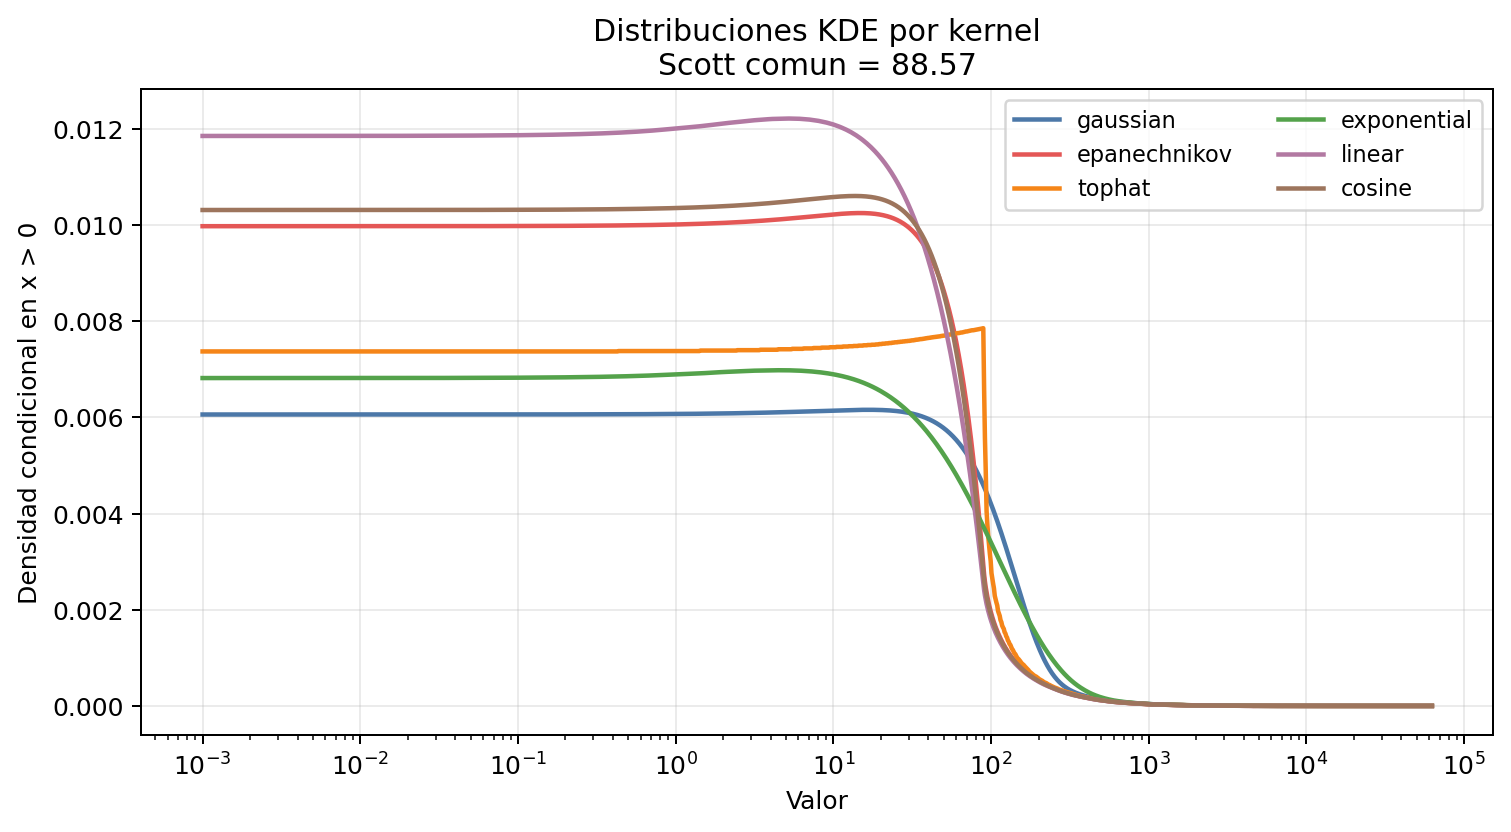
\includegraphics[width=0.82\textwidth]{../report_assets/kernel_common_scott_overlay.png}
\caption{Distribuciones KDE condicionales para los seis kernels con Scott absoluto comun.}
\end{figure}

\subsection{Distancias entre distribuciones de kernel}
La divergencia Jensen-Shannon y la distancia KS entre las distribuciones ajustadas muestran que no
todos los kernels se parecen entre si bajo el mismo Scott. Los pares mas cercanos son:
\begin{itemize}[leftmargin=1.5em]
\item \texttt{epanechnikov} vs \texttt{cosine}: JS \(=0.00010\), KS \(=0.0119\)
\item \texttt{linear} vs \texttt{cosine}: JS \(=0.00085\), KS \(=0.0341\)
\item \texttt{epanechnikov} vs \texttt{linear}: JS \(=0.00148\), KS \(=0.0451\)
\end{itemize}

Los pares mas distintos son:
\begin{itemize}[leftmargin=1.5em]
\item \texttt{gaussian} vs \texttt{linear}: JS \(=0.04364\), KS \(=0.2525\)
\item \texttt{exponential} vs \texttt{linear}: JS \(=0.04267\), KS \(=0.2602\)
\item \texttt{gaussian} vs \texttt{cosine}: JS \(=0.03847\), KS \(=0.2383\)
\end{itemize}

\begin{figure}[H]
\centering
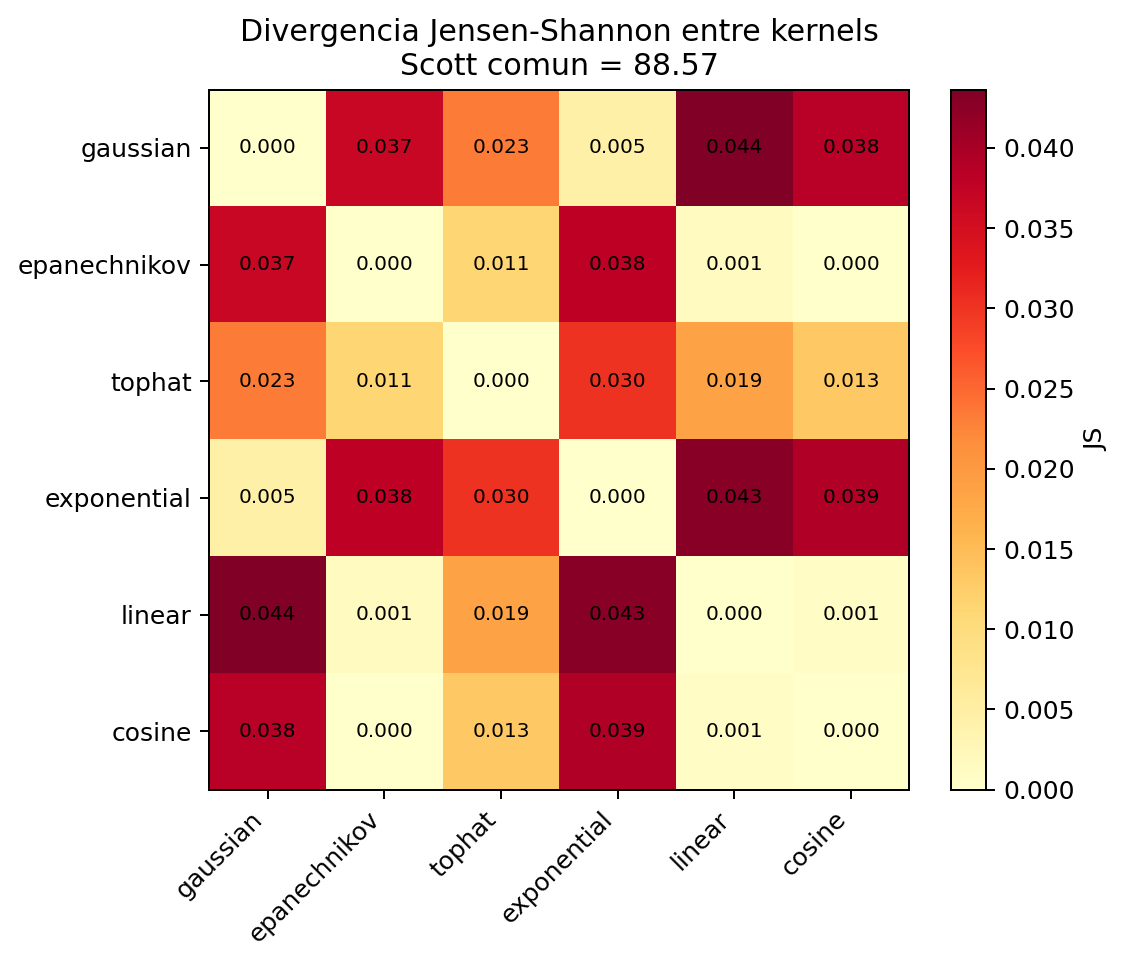
\includegraphics[width=0.72\textwidth]{../report_assets/kernel_pairwise_js_heatmap.png}
\caption{Mapa de calor de divergencias Jensen-Shannon entre kernels con Scott comun.}
\end{figure}

\subsection{Comparacion enfocada en los kernels realmente usados}
La comparacion mas importante para el flujo actual no es ``los seis kernels con Scott comun'', sino
los dos kernels que hoy tienen peso real en el proyecto:
\begin{itemize}[leftmargin=1.5em]
\item \texttt{gaussian} con Scott \(=88.57\), como baseline tecnico;
\item \texttt{epanechnikov} con CV \(=4.42837\), como opcion descriptiva actual en el notebook
      multikernel.
\end{itemize}

\begin{table}[H]
\centering
\caption{Kernels actualmente usados en el flujo}
\label{tab:active-kernels}
\begin{tabular}{lrrrr}
\toprule
Kernel & Bandwidth & Masa en \(x>0\) & Moda & KS \\
\midrule
gaussian     & 88.5675 & 0.6233 & 16.70 & 0.5494 \\
epanechnikov & 4.4284  & 0.9232 & 2.87  & 0.1409 \\
\bottomrule
\end{tabular}
\end{table}

La diferencia entre ambas distribuciones no es menor: para este par, la divergencia
Jensen-Shannon es \(0.1832\), la distancia KS entre CDFs es \(0.5126\) y la distancia \(L_1\)
es \(1.0387\). En otras palabras, no son dos variantes casi equivalentes; estan describiendo
regimenes de suavizado realmente distintos.

\begin{figure}[H]
\centering
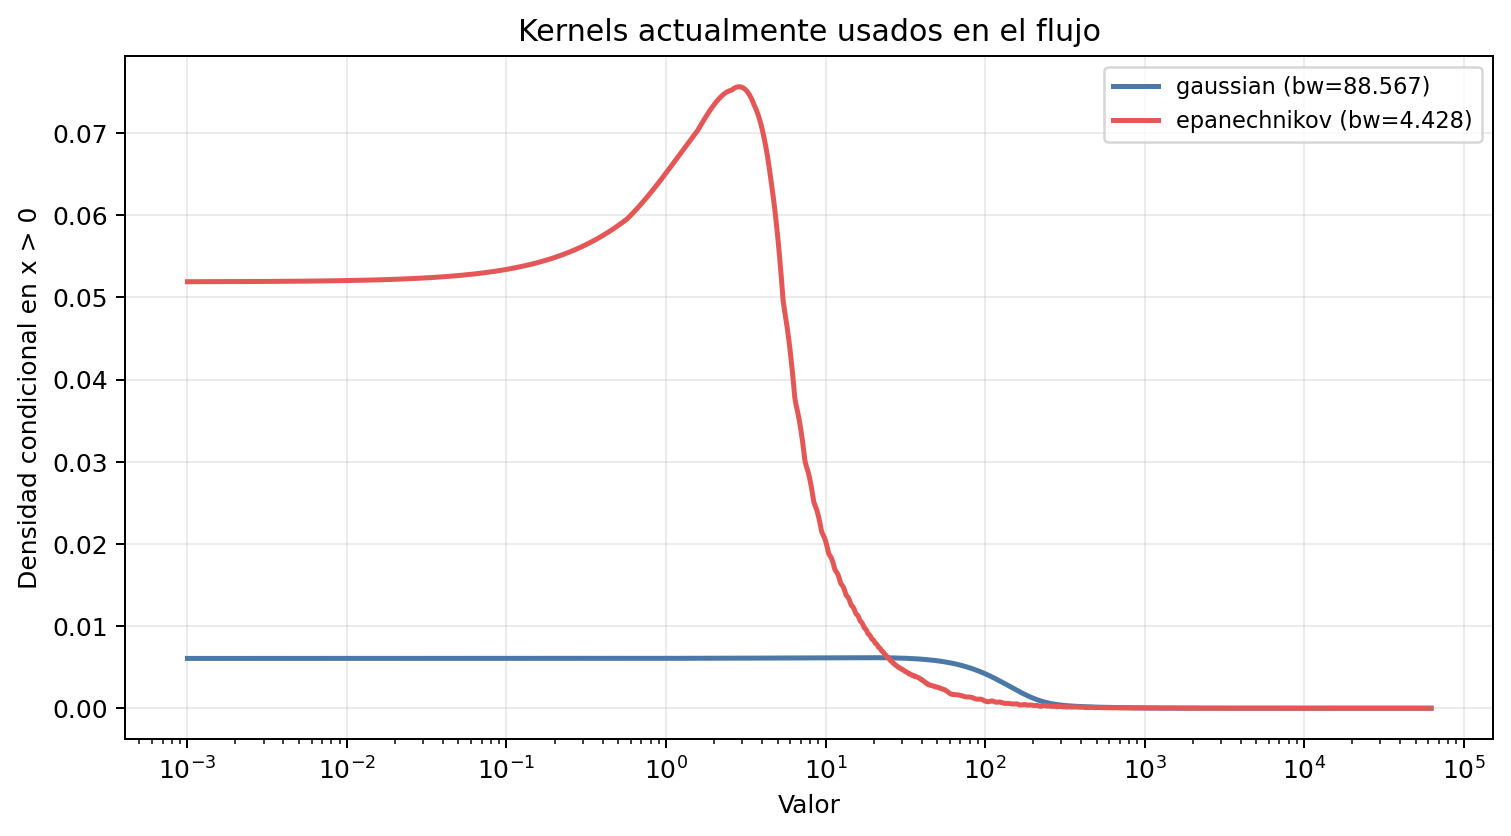
\includegraphics[width=0.82\textwidth]{../report_assets/kernel_active_overlay.png}
\caption{Comparacion de los dos kernels actualmente mas relevantes en el flujo.}
\end{figure}

\section{Correcciones concretas al PDF anterior}
La version previa quedaba corta en cuatro puntos y aqui se corrigen explicitamente:
\begin{enumerate}[leftmargin=1.5em]
\item El factor canonico del kernel \texttt{exponential} no es \(1.0\), sino \(0.73977\) respecto
      a Gaussian.
\item El factor de \texttt{cosine} debe tomarse como \(2.27498\), no \(2.2627\).
\item El resultado ``\texttt{gridsize\_opt = 10,000}'' no debe usarse como prueba de fallo del
      bandwidth; el test esta saturado en el rango explorado.
\item El kernel gaussiano con Scott es util como referencia tecnica, pero desplaza mucha masa a
      \(x<0\), por lo que no es el mejor resumen descriptivo si el dominio relevante es estrictamente
      positivo.
\end{enumerate}

\section{Recomendacion final}
Si la meta inmediata es dejar un flujo claro y utilizable, la recomendacion practica es:
\begin{enumerate}[leftmargin=1.5em]
\item Mantener \texttt{gaussian + Scott} como baseline de referencia y sanity check entre
      SciPy y scikit-learn.
\item Usar \texttt{epanechnikov + bw=4.42837} cuando el interes sea describir la distribucion de
      valores positivos con menor fuga de masa hacia \(x<0\).
\item Si se quiere comparar los seis kernels de forma mas justa, correrlos con los bandwidths
      canonicos de la Tabla~\ref{tab:bandwidths-canonicos}, no con un unico Scott absoluto.
\item Mantener \texttt{gridsize=10,000} como valor operativo por defecto para este pipeline, porque
      ya cumple el criterio de precision usado y reduce mucho el costo computacional.
\end{enumerate}

En sintesis, el proyecto queda mejor documentado si se presenta asi:
\begin{itemize}[leftmargin=1.5em]
\item \textbf{Gaussian + Scott}: referencia tecnica y compatibilidad historica.
\item \textbf{Epanechnikov + CV}: opcion descriptiva actualmente mas coherente con el soporte
      positivo de los datos.
\item \textbf{Resto de kernels}: utiles para comparacion, pero pendientes de una corrida sistematica
      con bandwidths comparables por kernel.
\end{itemize}

\section{Limitaciones abiertas}
Aunque el documento queda mucho mas fuerte que el PDF anterior, siguen abiertas tres limitaciones:
\begin{itemize}[leftmargin=1.5em]
\item se modela \(X \mid X > 0\), no la distribucion completa con ceros;
\item la unidad analizada sigue siendo la matriz aplanada, no una unidad biologica directa;
\item las conclusiones son validas como auditoria estadistica del pipeline KDE, no como inferencia
      biologica final sobre microbiota.
\end{itemize}

\begin{thebibliography}{9}
\bibitem{silverman}
B. W. Silverman.
\newblock \emph{Density Estimation for Statistics and Data Analysis}.
\newblock Chapman \& Hall, 1986.

\bibitem{scott}
D. W. Scott.
\newblock \emph{Multivariate Density Estimation: Theory, Practice, and Visualization}.
\newblock Wiley, 1992.

\bibitem{wandjones}
M. P. Wand and M. C. Jones.
\newblock \emph{Kernel Smoothing}.
\newblock Chapman \& Hall/CRC, 1995.
\end{thebibliography}

\end{document}
